\section{Results}\label{sec:Results}      

As defined in \textbf{chapter \ref{subsec:Performance_Assessment}} and \textbf{chapter \ref{subsec:Fairness_Assessment}}, each outcome is assessed in terms of performance and fairness with two pre-defined metric sets. Additionally, the aspect of Explainability will be demonstrated examplarily for the initial model run.

\subsection{Initial Performance}\label{subsec:Initial_Performance}

The initial run serving as a benchmark was conducted training the neural network described in \textbf{chapter \ref{subsec:Model_Training_and_Prediction}} on the unadjusted training data (see \textbf{chapter \ref{subsec:HMDA_Data}}).

\textbf{Explainability}

As was intended in \textbf{chapter \ref{subsec:Explainability}}, three different Explainability algorithms were utilized to challenge each other's results and analyze overall patterns. \textbf{figure \ref{fig:SHAP_explanations}} and \textbf{figure \ref{fig:LIME_explanations}} show the individual explanations for the first 150 observations of the test set provided by SHAP and LIME, respectively. 
As already mentioned in \textbf{chapter \ref{subsec:Performance_Assessment}}, the model behaved somewhat different from the expectations: Imputation of missing values in the \textit{debt\_to\_income\_ratio} feature led to a significant decrease in both fairness and performance measures of the model.
Therefore, it must be assumed that missingness in itself is not completely at random and holds information (or that the imputation method via a random forest regressor is not suitable for this task).
While SHAP considers that missingness to be the most important influence on model predictions, LIME weighs the \textit{debt\_to\_income\_ratio} features higher in general.
None of the algorithms consider the protected attributes to be of high direct impact on the results.

\begin{figure}[h]
    \centering
    \begin{minipage}{0.5\textwidth}
        \centering
        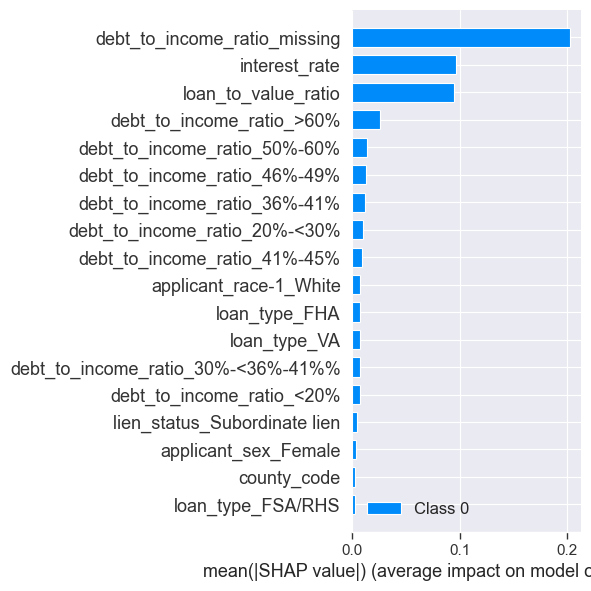
\includegraphics[width=\textwidth,height=5cm,keepaspectratio]{images/CHXX_UPDATE_SHAP_individual.png}
        \caption{SHAP individual explanations}
        \label{fig:SHAP_explanations}
    \end{minipage}\hfill
    \begin{minipage}{0.5\textwidth}
        \centering
        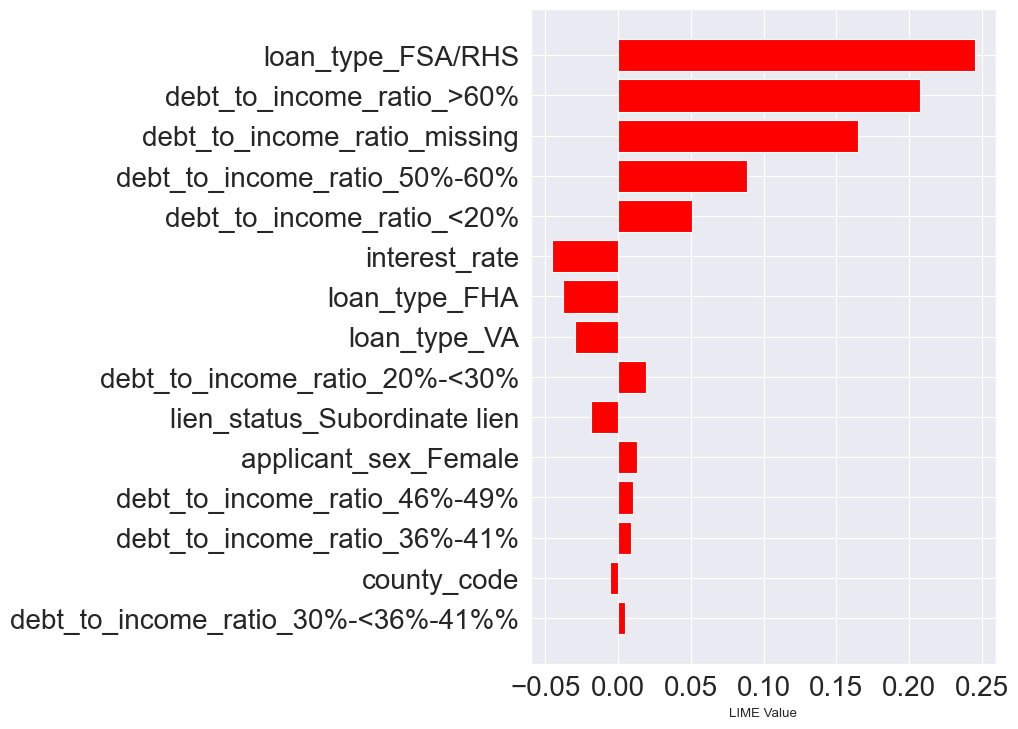
\includegraphics[width=\textwidth,height=5cm,keepaspectratio]{images/CHXX_UPDATE_LIME_individual.png}
        \caption{LIME individual explanations}
        \label{fig:LIME_explanations}
    \end{minipage}
    \caption*{Directly comparing LIME and SHAP explanations for the first 150 observations of the test set: While \textit{debt\_to\_income\_ratio} is an important factor in both explanations, its actual impact varies, as LIME also considers the \textit{loan\_type} feature to be of high importance. Default plotting options were kept: SHAP values are displayed as absolutes, while LIME values show the direction of their impact.}
\end{figure}

While the overall trends are similar with both algorithms, the actual impact of the features varies significantly. While this is not a direct threat to the quality of the results of this thesis, it is a reminder that Explainability algorithms need to be analyzed carefully. 
This ties with the findings of Krishna et al. \parencite{Krishna2022}, who emphasize the importance of understanding the underlying assumptions of Explainability algorithms and the need for a more comprehensive evaluation of their results.

To validate the results of the local explanations, a \textit{Global Surrogate Model} was used. \textbf{figure \ref{fig:Global_Surrogate}} shows the results of the global surrogate model. Specifically, the five most important features according to the global surrogate model are compared to the SHAP and LIME explanations in terms of their relative performance.
It is apparent that the overall trends of SHAP and LIME are close to the global explanations.

\begin{figure}[h]
    \centering
    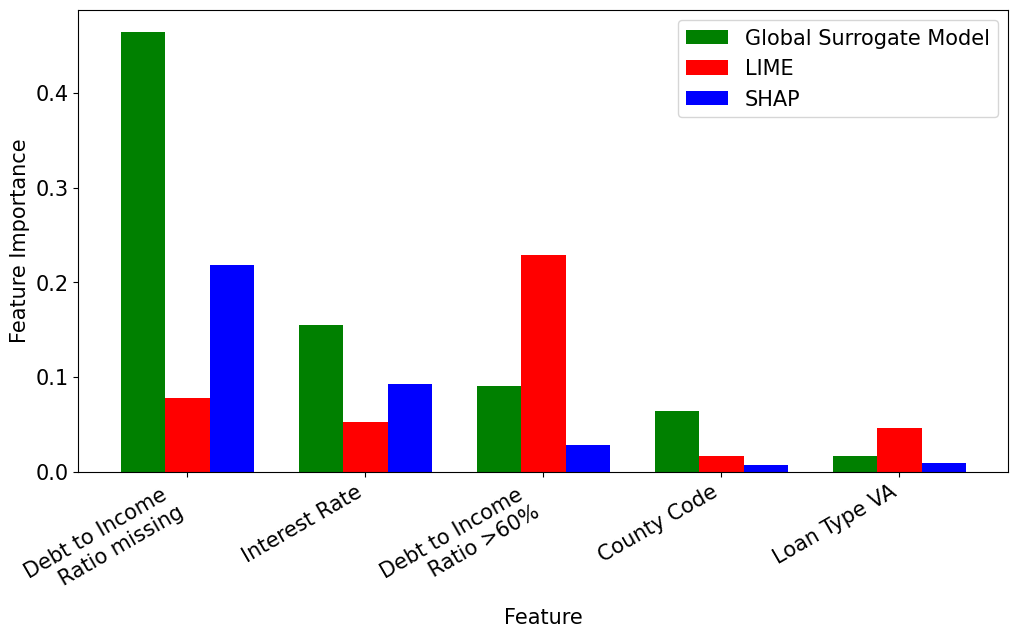
\includegraphics[width=0.85\textwidth]{images/CHXX_UPDATE_Surrogate_SHAP_LIME_combined.png}
    \caption{Global Surrogate Model compared to SHAP and LIME}
    \caption*{Analyzing the 5 most important features according to the global surrogate model implies that the overall trends of SHAP and LIME are close to the global explanations.}
    \label{fig:Global_Surrogate}
\end{figure}

\textbf{Performance}

Even without directly comparable benchmarks available (see \textbf{chapter \ref{subsec:Performance_Assessment}}), the initial model performance can be considered as good. Details can be found in \textbf{table \ref{tab:initial_model_performance_results_1}}.

\begin{table}[h]
    \centering
    \begin{tabular}{l c}
    \toprule
    \textbf{Metric} & \textbf{Value} \\
    \midrule
    \textbf{accuracy} & 0.90 \\
    \textbf{precision} & 0.88 \\
    \textbf{recall} & 0.96 \\
    \textbf{f1} & 0.92 \\
    \textbf{roc\_auc} & 0.94 \\
    \bottomrule
    \end{tabular}
    \caption{Metrics \#1: Initial Model}
    \caption*{The initial model shows a high accuracy and recall, but a lower precision and f1 score. The overall performance can be considered good.}
    \label{tab:initial_model_performance_results_1}
\end{table}

\textbf{Fairness}

\textbf{Table \ref{tab:initial_model_fairness_results_1}} shows the results of the fairness assessment of the initial model. The disparities in the true positive rate and false positive rate are relatively low, while the disparities in the true negative rate and false negative rate are higher.

\begin{table}[h]
    \caption{Metrics \#2: Initial Model}
    \begin{minipage}[t]{0.5\textwidth}
    \centering
    \begin{tabular}{lr}
    \toprule
    \textbf{Metric} & \textbf{Value} \\
    \midrule
    \textbf{Accuracy White} & 0.91 \\
    \textbf{Precision White} & 0.89 \\
    \textbf{Recall White} & 0.97 \\
    \textbf{F1 Score White} & 0.93 \\
    \textbf{AUC White} & 0.94 \\
    \textbf{Accuracy Black} & 0.89 \\
    \textbf{Precision Black} & 0.84 \\
    \textbf{Recall Black} & 0.92 \\
    \textbf{F1 Score Black} & 0.88 \\
    \textbf{AUC Black} & 0.95 \\
    \bottomrule
    \end{tabular}
    \end{minipage}\hfill
    \begin{minipage}[t]{0.5\textwidth}
    \centering
    \begin{tabular}{lr}
    \toprule
    \textbf{Metric} & \textbf{Value} \\
    \midrule
    \textbf{tpr\_disparity} & 0.95 \\
    \textbf{fpr\_disparity} & 0.77 \\
    \textbf{tnr\_disparity} & 1.05 \\
    \textbf{fnr\_disparity} & 2.51 \\
    \bottomrule
    \end{tabular}
    \end{minipage}
    \label{tab:initial_model_fairness_results_1}
    \caption*{The initial model shows a higher accuracy and recall for White applicants, but a higher precision and F1 score for Black applicants. The AUC is higher for Black applicants. The disparities in the true positive rate and false positive rate are relatively low, while the disparities in the true negative rate and false negative rate are higher.}
\end{table}

\subsection{Results of the Iterations}\label{subsec:Iterations}

None of the techniques applied in the iterations led to a significant increase in fairness. The \textit{reweighing} technique managed to improve the overall fairness of the model, but the other techniques did not manage to reach the same level of fairness. 
Figures \textbf{\ref{fig:Initial_Disparity}} to \textbf{\ref{fig:Calibrated_EqOdds_Disparity}} show that the disparity in loan grants between \textit{White} and \textit{Black or African American} applicants was not substantially reduced by any of the iterations, with the calibrated equalized odds algorithm even increasing the disparity.

\begin{figure}[h]
    \centering
    \begin{minipage}{0.5\textwidth}
        \centering
        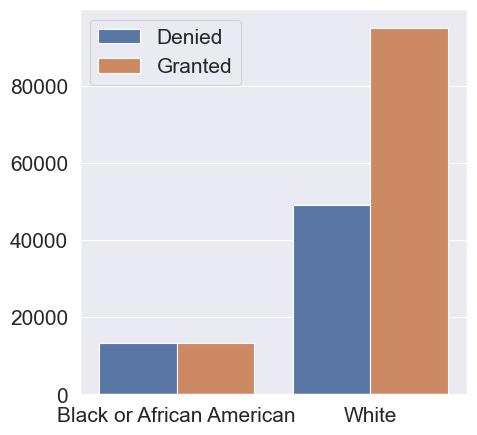
\includegraphics[width=\textwidth]{images/loan_grants_by_protected_attributes/initial.png}
        \caption{Initial Model Disparity}
        \label{fig:Initial_Disparity}
    \end{minipage}\hfill
    \begin{minipage}{0.5\textwidth}
        \centering
        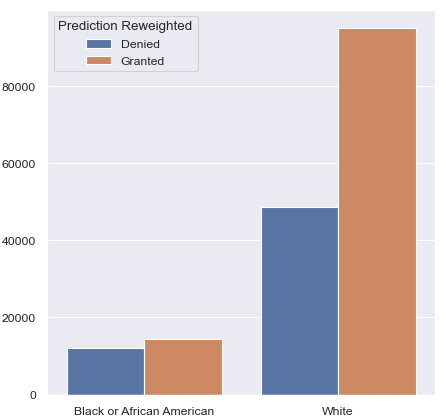
\includegraphics[width=\textwidth]{images/loan_grants_by_protected_attributes/reweighted.png}
        \caption{Reweighed Model Disparity}
        \label{fig:Reweighed_Disparity}
    \end{minipage}
    
    \vspace{1em} 
    
    \begin{minipage}{0.5\textwidth}
        \centering
        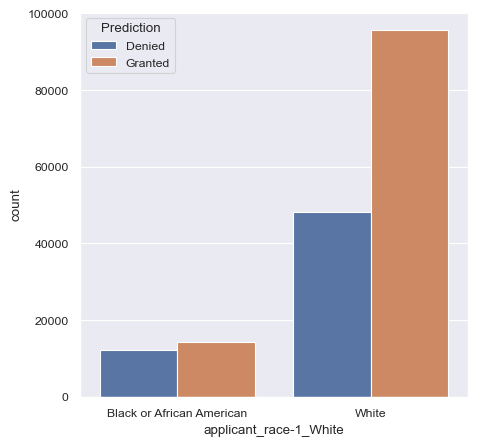
\includegraphics[width=\textwidth]{images/loan_grants_by_protected_attributes/correlation_removed.png}
        \caption{Corr. Rem. Model Disparity}
        \label{fig:Correlation_Removed_Disparity}
    \end{minipage}\hfill
    \begin{minipage}{0.5\textwidth}
        \centering
        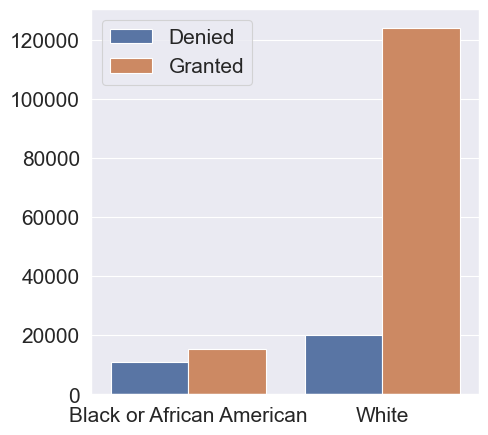
\includegraphics[width=\textwidth]{images/loan_grants_by_protected_attributes/calibrated_eqodds.png} 
        \caption{Cal. Eq. Odds Model Disparity}
        \label{fig:Calibrated_EqOdds_Disparity}
    \end{minipage}
    
    \label{fig:Racial_Disparities}
    \caption*{Apart from the Calibrated Equalized Odds model, which exhibits a higher amount of overall predicted grants, none of the iterations were able to substantially reduce the disparity in granted loans between races.}
\end{figure}

In terms of \textbf{performance}, the iterations did not lead to a significant increase in performance, with the \textit{Calibrated Equalized Odds} model even showing a significant decrease in performance. \textbf{Table \ref{tab:metrics_1_iterations}} shows the results of the performance assessment of the iterations.
All iterations tended to be closer to each other than expected. The best value (which is marked in bold), was only achieved at the third or fourth digit after the comma in many cases, leading to changes in the "best" model across different iterations.

\begin{table}[h]
    \centering
    \caption{Metrics \#1: Iterations}
    \begin{tabular}{l *{4}{>{$}c<{$}}}
    \toprule
    & \textbf{Initial Model} & \textbf{Reweighing} & \textbf{Calibrated Equalized Odds} & \textbf{Correlation Removal} \\
    \midrule
    \textbf{accuracy} & 0.90 & 0.90 & 0.73 & \textbf{0.91} \\
    \textbf{precision} & 0.88 & 0.88 & 0.69 & \textbf{0.88} \\
    \textbf{recall} & 0.96 & \textbf{0.97} & 0.97 & 0.97 \\
    \textbf{f1} & 0.92 & 0.92 & 0.81 & \textbf{0.92} \\
    \textbf{roc\_auc} & \textbf{0.94} & 0.94 & \text{NA} & \text{NA} \\
    \bottomrule
    \end{tabular}
    \caption*{Except the Calibrated Equalized Odds Model, all iterations show a similar performance to the initial model. The Correlation Removal Model shows a slightly higher accuracy and f1 score.}
    \label{tab:metrics_1_iterations}
\end{table}

Similarly to the performance, the iterations did not lead to a significant increase in (subgroup) fairness. The \textit{reweighing} technique managed to improve the overall fairness of the model, but the other techniques did not manage to reach the same level of fairness. \textbf{Table \ref{tab:metrics_2_1_iterations}} shows the results of the fairness assessment of the iterations for the first part of \textit{metrics \#2}.

\begin{table}[h]
    \centering
    \caption{Metrics \#2 (1): Iterations}
    \begin{tabular}{l *{4}{>{$}c<{$}}}
    \toprule
    & \textbf{Initial Model} & \textbf{Reweighing} & \textbf{Calibrated Equalized Odds} & \textbf{Correlation Removal} \\
    \midrule
    \textbf{Accuracy White} & 0.91 & 0.91 & 0.72 & \textbf{0.91} \\
    \textbf{Precision White} & \textbf{0.89} & 0.89 & 0.68 & 0.89 \\
    \textbf{Recall White} & 0.97 & 0.97 & \textbf{0.98} & 0.98 \\
    \textbf{F1 Score White} & 0.93 & 0.92 & 0.81 & \textbf{0.93} \\
    \textbf{AUC White} & \textbf{0.94} & 0.94 & \text{NA} & \text{NA} \\
    \midrule
    \textbf{Accuracy Black} & \textbf{0.89} & 0.88 & 0.81 & 0.88 \\
    \textbf{Precision Black} & 0.84 & 0.81 & 0.73 & \textbf{0.85} \\
    \textbf{Recall Black} & 0.92 & \textbf{0.97} & 0.93 & 0.92 \\
    \textbf{F1 Score Black} & 0.88 & \textbf{0.88} & 0.82 & 0.88 \\
    \textbf{AUC Black} & 0.95 & \textbf{0.95} & \text{NA} & \text{NA} \\
    \bottomrule
    \end{tabular}
    \caption*{Once again, the Calibrated Equalized Odds Model shows a significant decrease in performance. The other models show a similar performance to the initial model.}
    \label{tab:metrics_2_1_iterations}
\end{table}

In terms of disparities (see \textbf{table \ref{tab:metrics_2_2_iterations}}), the \textit{reweighing} technique managed to improve the overall fairness of the model, but the other techniques did not manage to reach the level of the initial model.
While across different model runs the disparities for the iterated models were very comparable, with the \textit{reweighing} technique consistently outperformung the other iterations, the performance in terms of disparities of the initial model varied strongly across different runs.

\begin{table}[h]
    \centering
    \caption{Metrics \#2 (2): Iterations}
    \begin{tabular}{l *{4}{>{$}c<{$}}}
    \toprule
    & \textbf{Initial Model} & \textbf{Reweighing} & \textbf{Calibrated Equalized Odds} & \textbf{Correlation Removal} \\
    \midrule
    \textbf{tpr\_disparity} & 0.95 & \textbf{1.00} & 0.95 & 0.94 \\
    \textbf{fpr\_disparity} & 0.77 & \textbf{1.00} & 0.43 & 0.76 \\
    \textbf{tnr\_disparity} & 1.01 & \textbf{1.00} & 2.23 & 1.06 \\
    \textbf{fnr\_disparity} & 2.51 & \textbf{0.84} & 3.25 & 3.42 \\
    \bottomrule
    \end{tabular}
    \caption*{In terms of disparities, the positive effects of reweighing show, with the algorithm outperforming the other iterations.}
    \label{tab:metrics_2_2_iterations}
\end{table}

Visualizing the results of the iterations in a comparison chart (\textbf{figure \ref{fig:Fairness_Comparison_Chart}}) shows that while the initial model managed to put out values with a comparably high fairness as measured by disparities, reweighing managed to improve this overall performance. The other two models however did not manage to reach the same level of fairness.

\begin{figure}
    \centering
    \caption{Fairness Comparison Chart}
    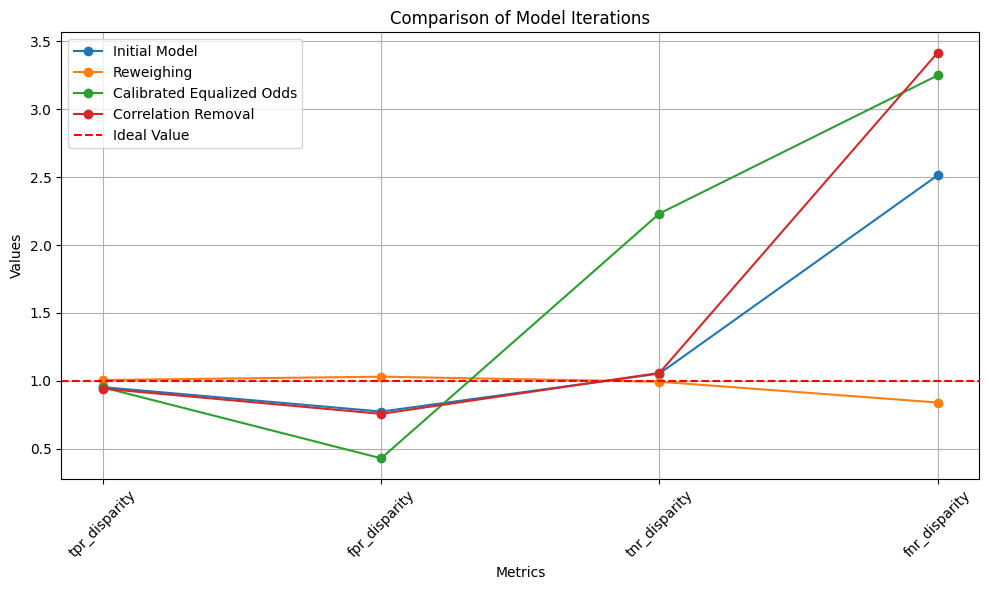
\includegraphics[width=0.85\textwidth]{images/CHXX_UPDATE_Results_Line.png}
    \caption*{While the initial model managed to put out values with a comparably high fairness as measured by disparities, reweighing managed to improve this overall performance. The other two models however did not manage to reach the same level of fairness.}
    \label{fig:Fairness_Comparison_Chart}
\end{figure}

% \section{Limitations}\label{sec:Limitations} - hier oder am Ende?
